\section{Definice ovládání, řízení a regulace(řízení bez a se zpětnou vazbou),výhody a nevýhody.Základní veličiny a přenosy. Rozdělení řízení podle různých kritérií. PID regulátory, základní složky a vlastnosti. Statistická analýza zpětnovazebních obvodů. Standartní přenosy ve zpětnovazebním řízení, charakteristický polynom. Věta o počáteční a konečné hodnotě, požadavky na ustálené hodnoty.}
\subsection*{Ovládání}
tj. bez zpětné vazby\\
bez znalosti skutečné hodnoty na výstupu, tím pádem nelze kompenzovat vliv poruchových signálů, nelze zajistit správné sledování v případě změn parametrů soustavy\\
\subsection*{Řízení}
se zpětnou vazbou, tím pádem regulační odchylka e - rozdíl mezi vstupem a výstupem 
\subsection*{Regulace}
Krom regulační odchylky je zde i regulátor, který generuje akční zásah na základě odchylky a poruchy.
\begin{figure}[H]
    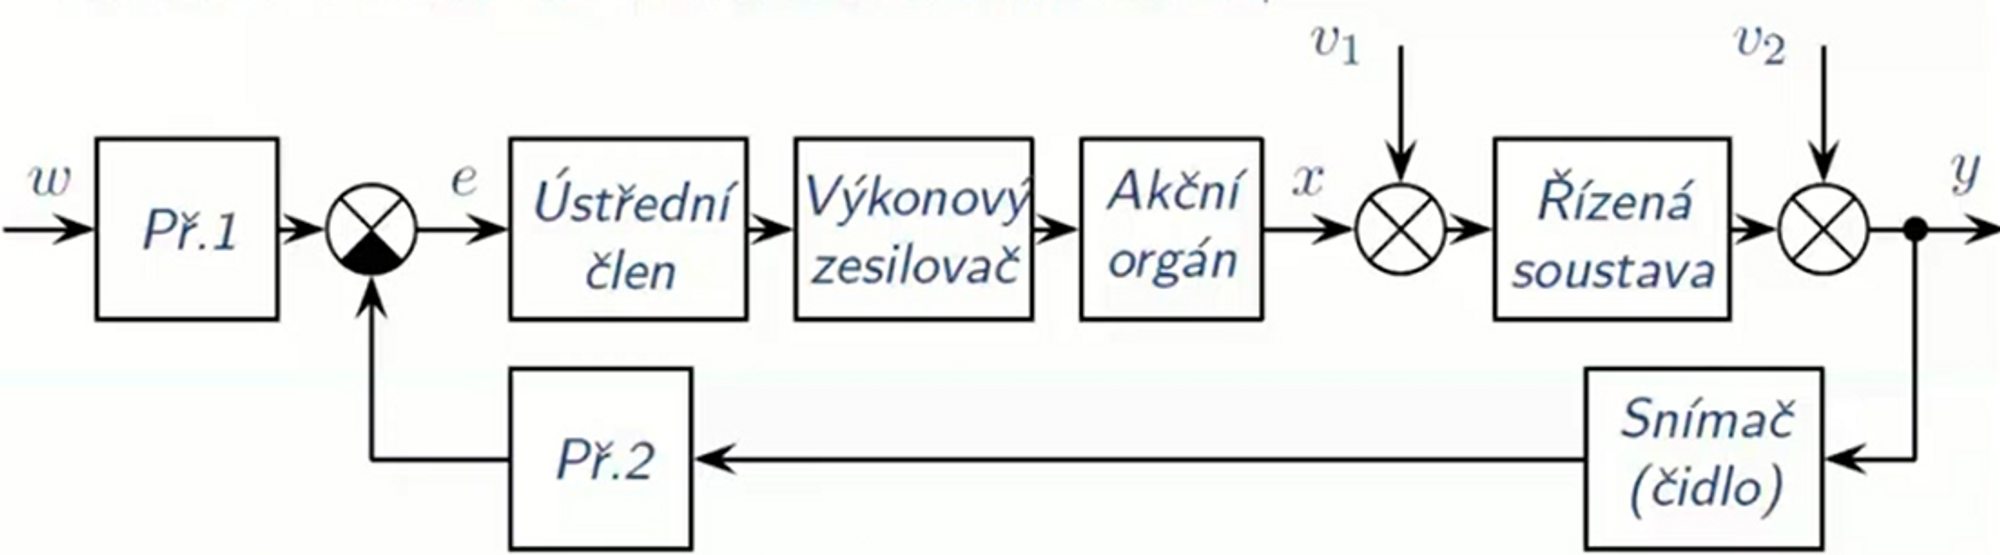
\includegraphics[scale = 0.45]{images/reg.soustava.png}
    \caption{Rozšířená regulačnní smyčka}
\end{figure}
\subsection*{Základní veličiny a přenosy}
\begin{figure}[H]
    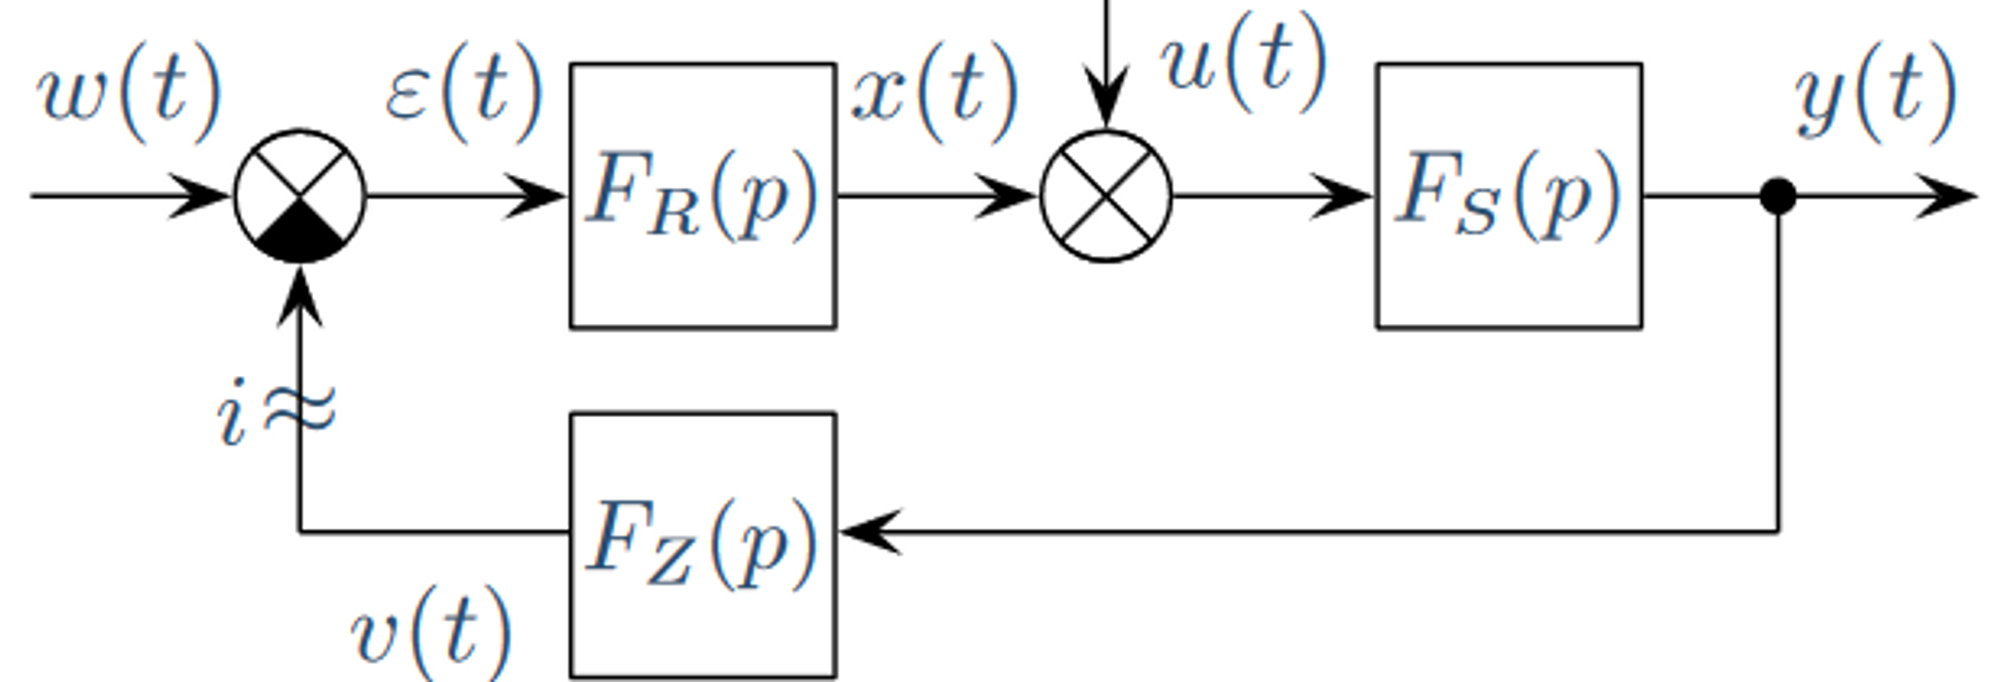
\includegraphics[scale = 0.45]{images/reg.soustava2.png}
    \caption{Regulačnní smyčka}
\end{figure}
w(t) \dots vstupní signál \\
$\epsilon(t)$ \dots odchylka \\
x(t) \dots akční veličina \\
u(t) \dots porucha \\
y(t) \dots výstupní signál\\
v(t) \dots výstup ze zpětné vazby\\
i    \dots výstup f0 za předpokladu, že je zpětná vazba rozpojená\\

\noindent
Přenos regulované soustavy:
\begin{equation}
    F_S(p) = \frac{Y(p)}{X(p)}
\end{equation}
Přenos regulátoru:
\begin{equation}
    F_R(p) = \frac{X(p)}{\epsilon(p)}
\end{equation}
Přenos zpětné vazby:
\begin{equation}
    F_Z(p) \frac{V(p)}{Y(p)}
\end{equation}
Otevřené smyčky:
\begin{equation}
    F_0(p) = \frac{Y(p)}{W(p)}
\end{equation}
Přenos řízení:
\begin{equation}
    F_W(p) = \frac{Y(p)}{W(p)}
\end{equation}
Přenos poruchy:
\begin{equation}
    F_U(p) = \frac{Y(p)}{U(p)}
\end{equation}
Přenos odchylky:
\begin{equation}
    F_E(p)=\frac{E(p)}{W(p)}
\end{equation}
Přenos akční veličiny:
\begin{equation}
    F_a(p) = \frac{X(p)}{W(p)}
\end{equation}
\subsection*{Rozdělení řízení podle kritérií}
Řízení na konstantní hodnotu:
\begin{itemize}
    \item obecně regulátory
    \item např. frekvence, napětí, hladina vody, teplota
\end{itemize}
Řízení hodnoty s neznámým průběhem
\begin{itemize}
    \item cíl zajistit co nejpřesnější a nejpřesnější sledování průběhu - obecně servomechanismus
    \item sledování polohy
\end{itemize}
Řízení na hodnoty s předem známým průběhem:
\begin{itemize}
    \item sledování výstupu a kompenzace poruch jsou rovnocenné
    \item lze použít řídící algoritmus - programově řízené
\end{itemize}
\subsection*{PID regulátor}
Obsahuje proporciální, integrační a derivační složku
\begin{equation}
    F_R(p) = K_R(1+T_Dp+\frac{1}{T_Ip}) = k_r\frac{(T_1p+1)(T_2p+1)}{p}
\end{equation}
proporciální složka == offset, větší zesílení, větší přesnost \\
integrační složka - zhoršuje dynamické vlastnosti, zpomaluje regulační děj, slouží k nulové ustálené odchylce nebo poruše\\
derivační složka - zlepšuje dynamické vlastnosti, zrychluje regulační děj, realizační konstanta zesiluje působení šumu\\
Pásmo proporcionality - udává, jaká je nutná změna ke změně výstupní veličiny regulátoru
\begin{equation}
    pp = \frac{1}{r_0}
\end{equation}
\begin{figure}[H]
    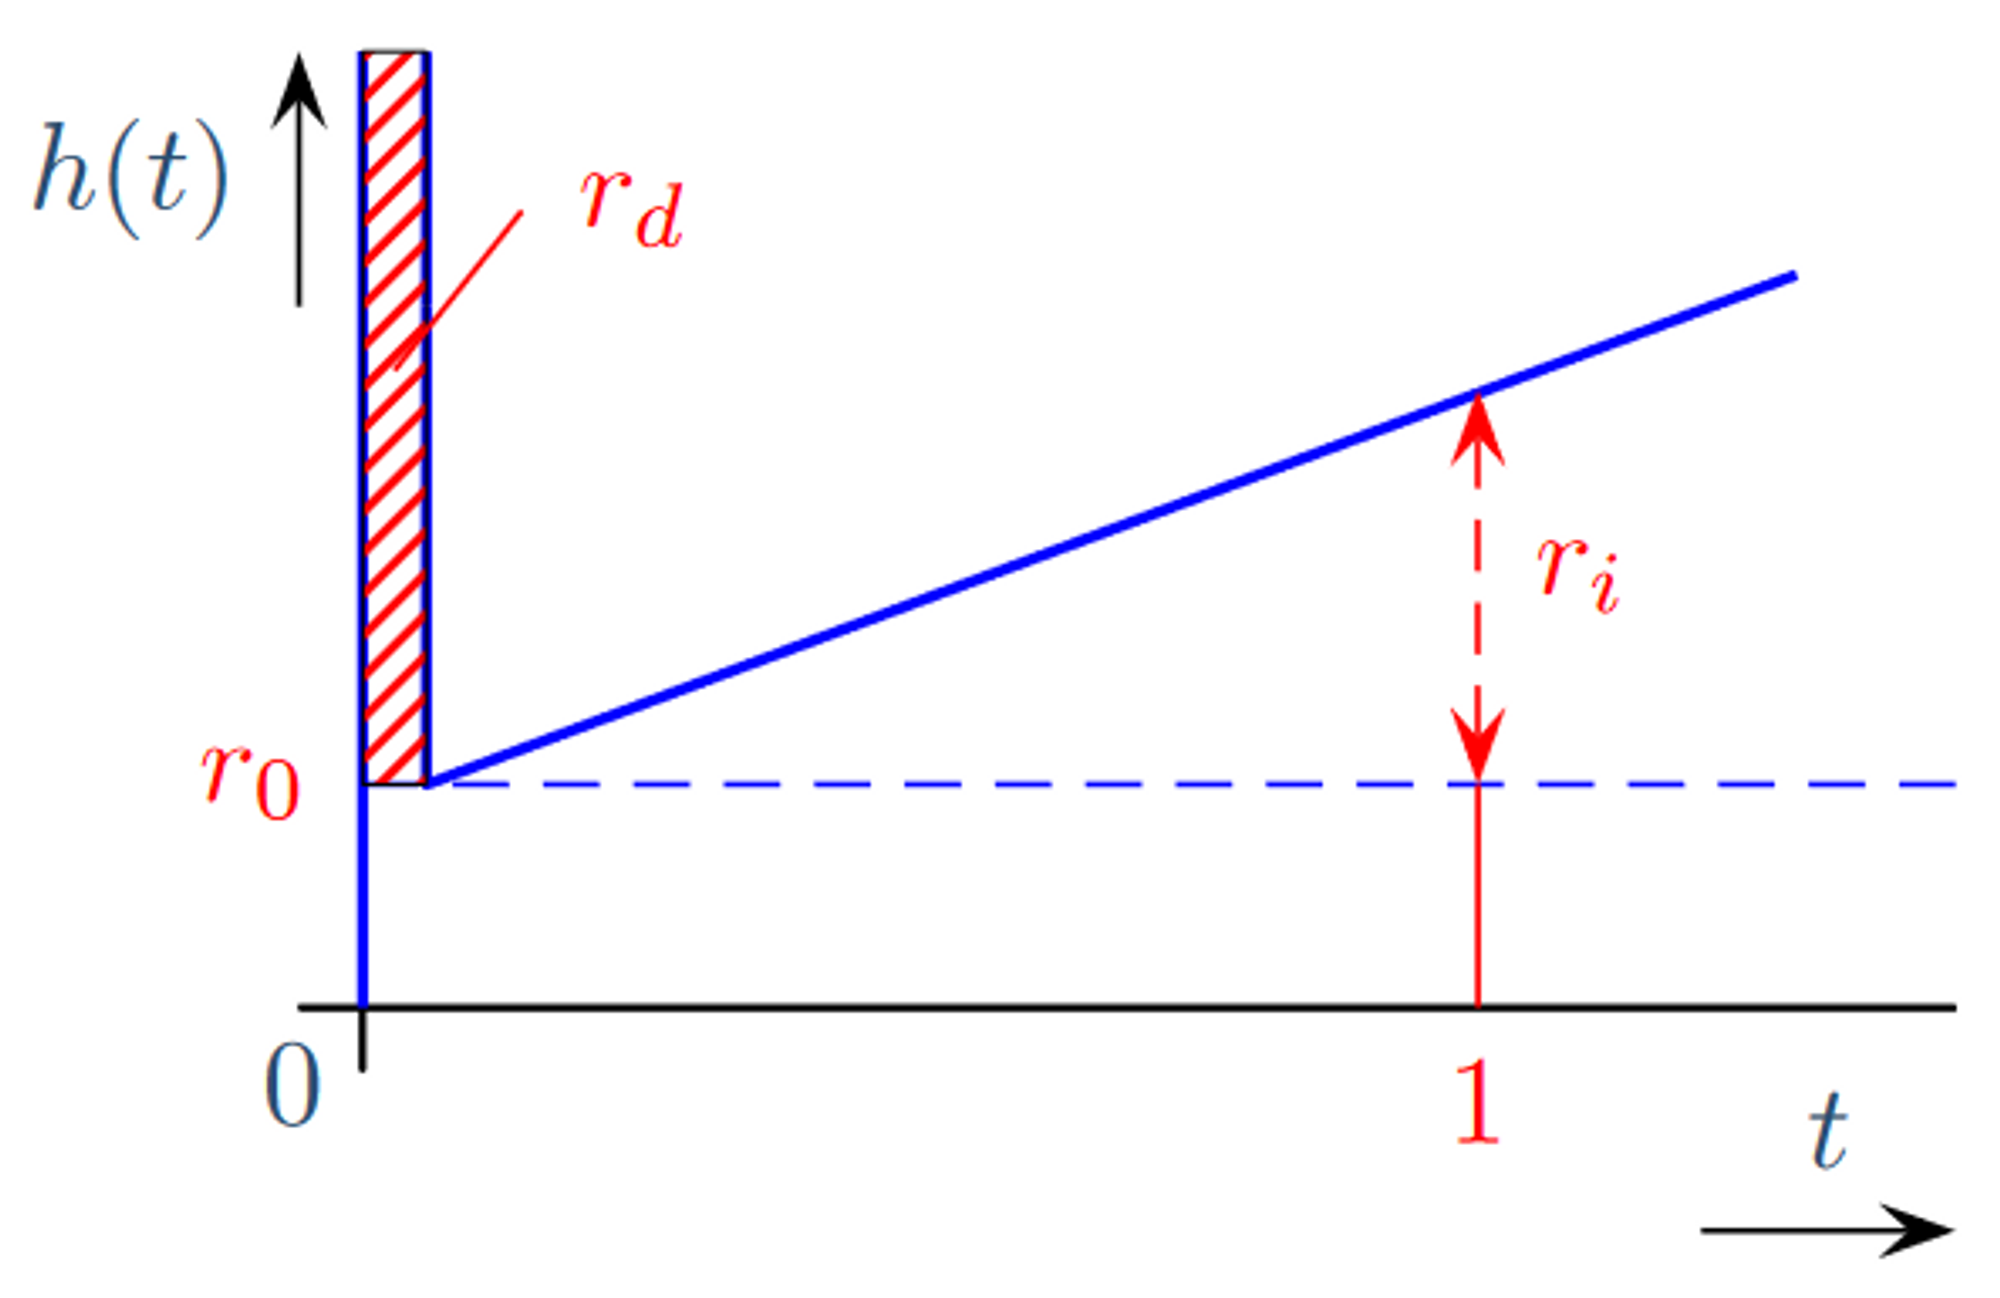
\includegraphics[scale = 0.3]{images/pasmo_proporcionality.png}
    \caption{PID}
\end{figure}
Rozdíl mezi reálným PID a PID:
\begin{itemize}
    \item reálný má realizační konstantu ve jmenovateli
    \item křivky jsou více zaoblené(viz obr. č. \ref{PID})
\end{itemize}
\begin{figure}[H]
    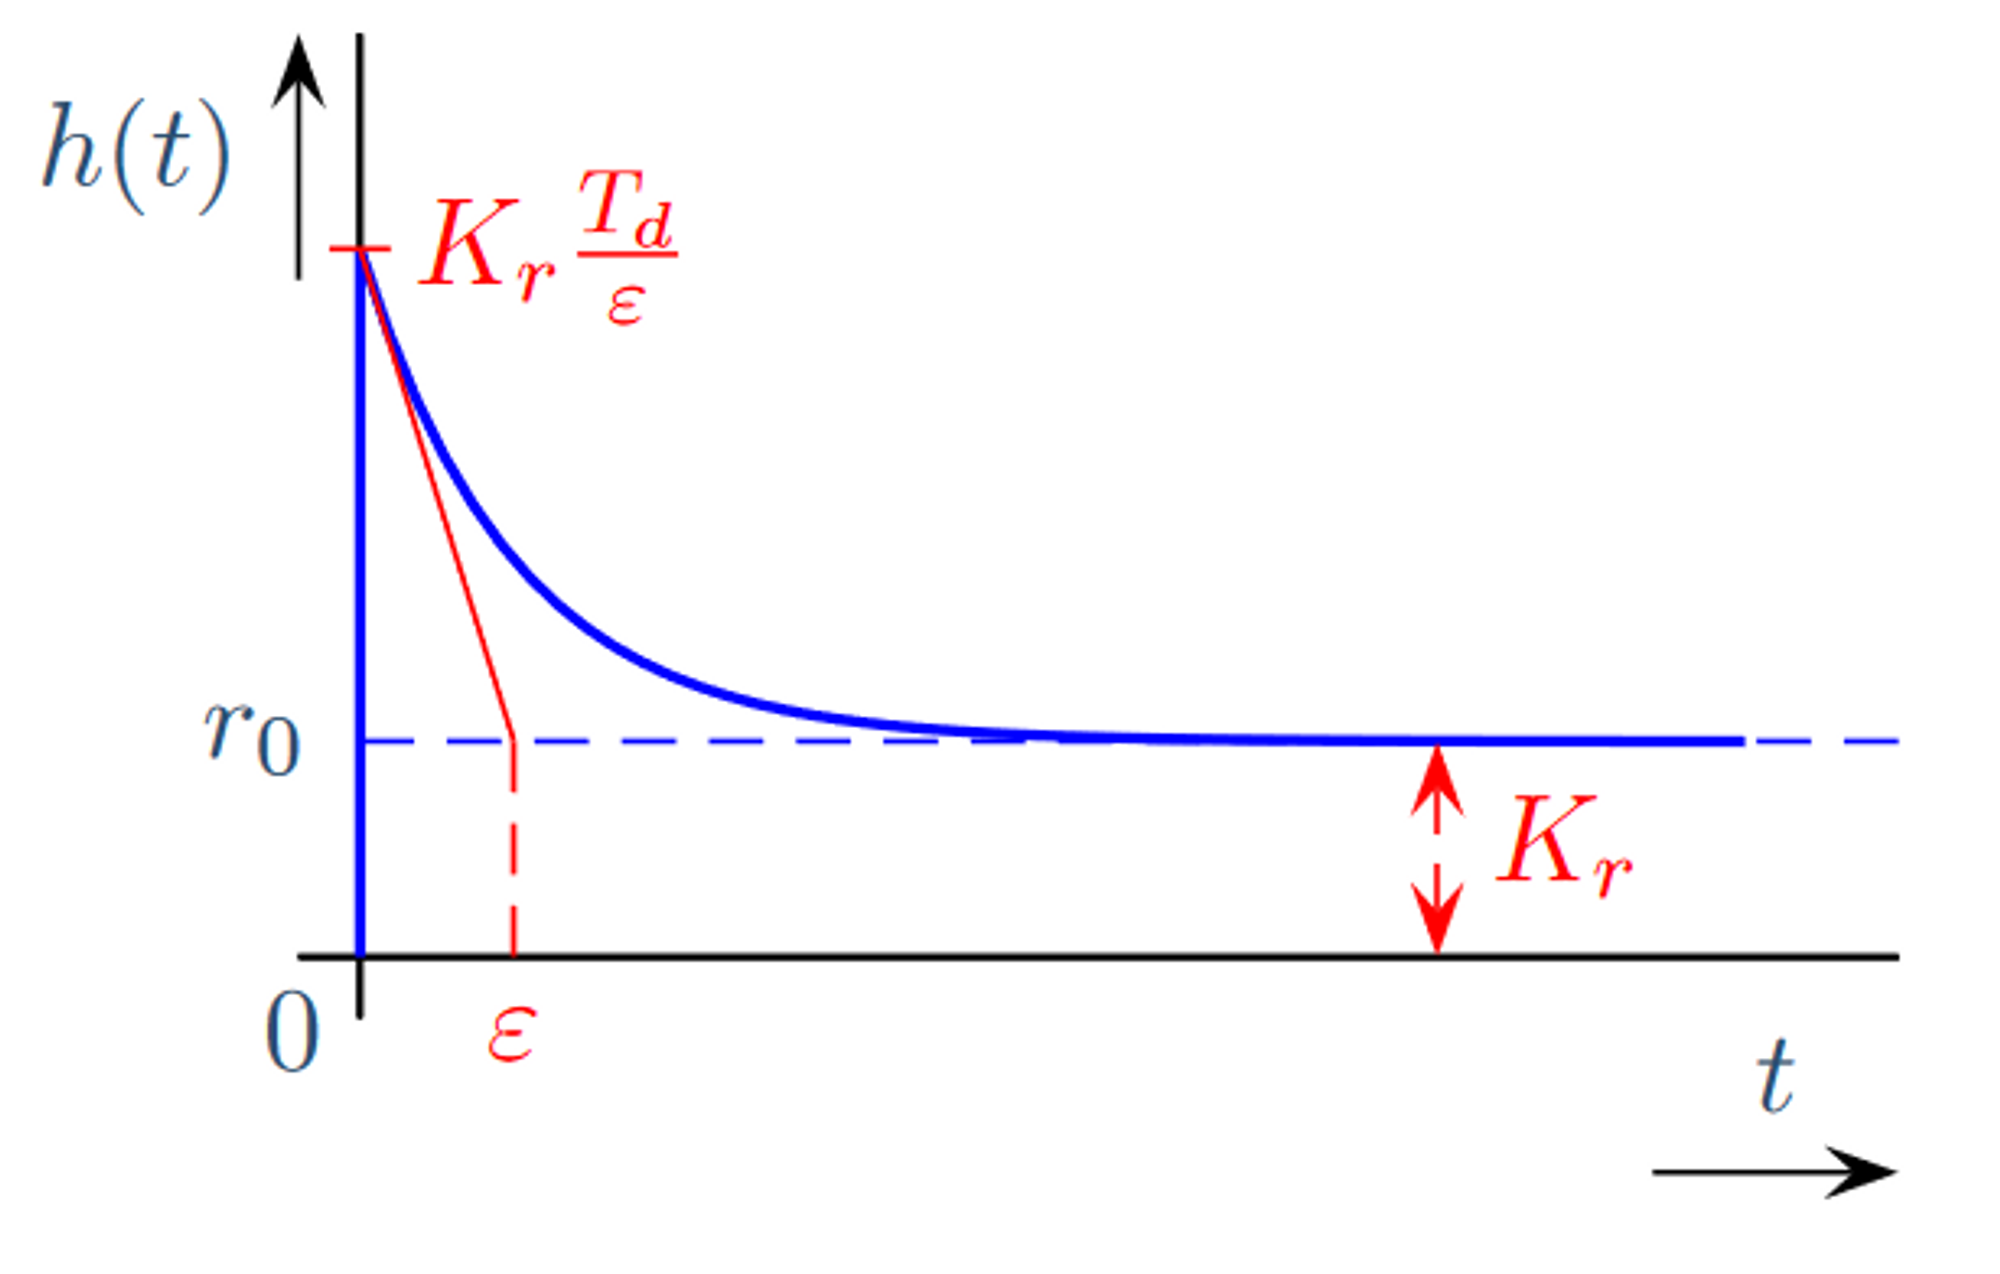
\includegraphics[scale = 0.3]{images/PID.png}
    \caption{Reálný PID}
    \label{PID}
\end{figure}
\subsection*{Statická analýza zpětnovazebních obvodů}
Přetlumené soustavy
\begin{itemize}
    \item bez kmitání
    \item sériové spojení setrvačných článků - všechny póly reálné a záporné
\end{itemize}
\begin{equation}
    F(p) =\frac{K}{(Tp+1)^n}
\end{equation}
\begin{figure}[H]
    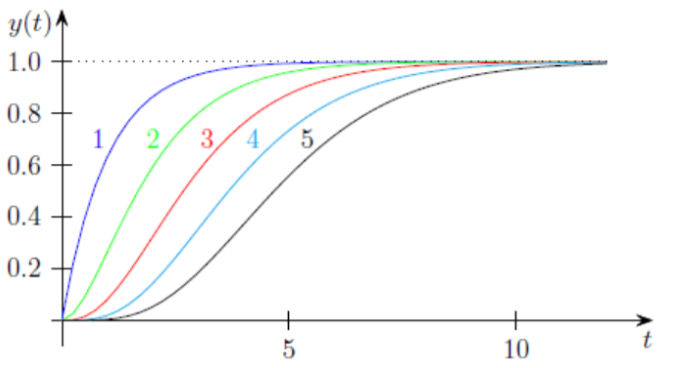
\includegraphics[scale = 1]{images/tlumeni.png}
    \caption{regulační křivky s rozdílným n}
\end{figure}
\newpage

Kmitavé soustavy:
\begin{itemize}
    \item v přenosové funkci se vyskytují komplexně sdružené póly
    \item v časových odezvách se nacházejí harmonické funkce sin a cos
    \item pokud kmitavé póly nejsou domunantní, kmitání nemusí být patrné
\end{itemize}
\begin{equation}
    F(p) = \frac{k}{(p^2+p+1)(0,1p+1)}
\end{equation}

Soustavy s astatismem:
\begin{itemize}
    \item přítomnost nezavazbeného integrátoru
    \item obsahují pól v počátku
    \item náchylné k nestabilitě
    \item přechodovka odchází do nekonečna
    \item zhoršuje vlastnosti řízení, ale nulová ustálená odchylka
\end{itemize}

Soustavy s neminimální fází:
\begin{itemize}
    \item jedna nebo více nul v pravé polorovině
    \item chová se divně . podkmit u jednotkového skoku na začátku
    \item ve frekvenčních charakteristikách neplatí vztah mezi sklonem a fází frekvenční charakteristiky
\end{itemize}

Soustavy s dopravním zpožděním:
\begin{itemize}
    \item $y(t) = x(t-d)$ v obraze $F(p) = e^{-dp}$
\end{itemize}
\newpage

\subsection*{Charakteristický polynom}
\begin{equation}
    1+F_0(p)
\end{equation}
Všechny přenosy uzavřeného obvodu mají ve jmenovateli tento tvar\\
když jsou jeho kořeny menší nule, je stabilní, pokud jsou rovny nule, tak je na mezi stability\\
\subsection*{Věta o počáteční a konečné hodnotě, požadavky na ustálené hodnoty}
\begin{figure}[H]
    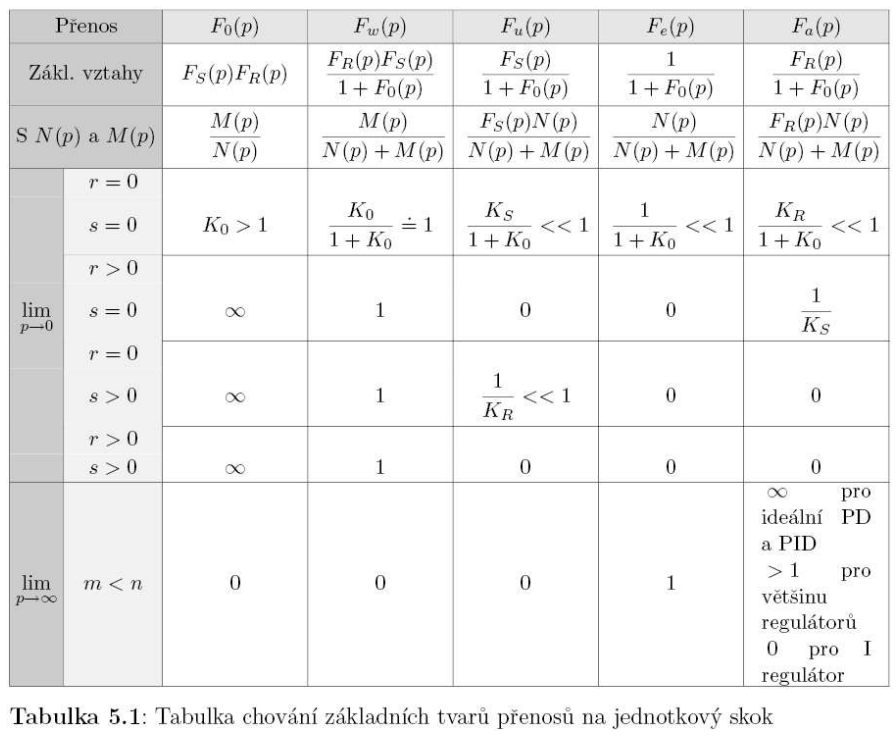
\includegraphics[scale = 0.8]{images/tvary_prenosu.png}
\end{figure}
Ustálená odchylka pro různé vstupy a počet integrátorů v soustavě a regulátoru:
\begin{figure}[H]
    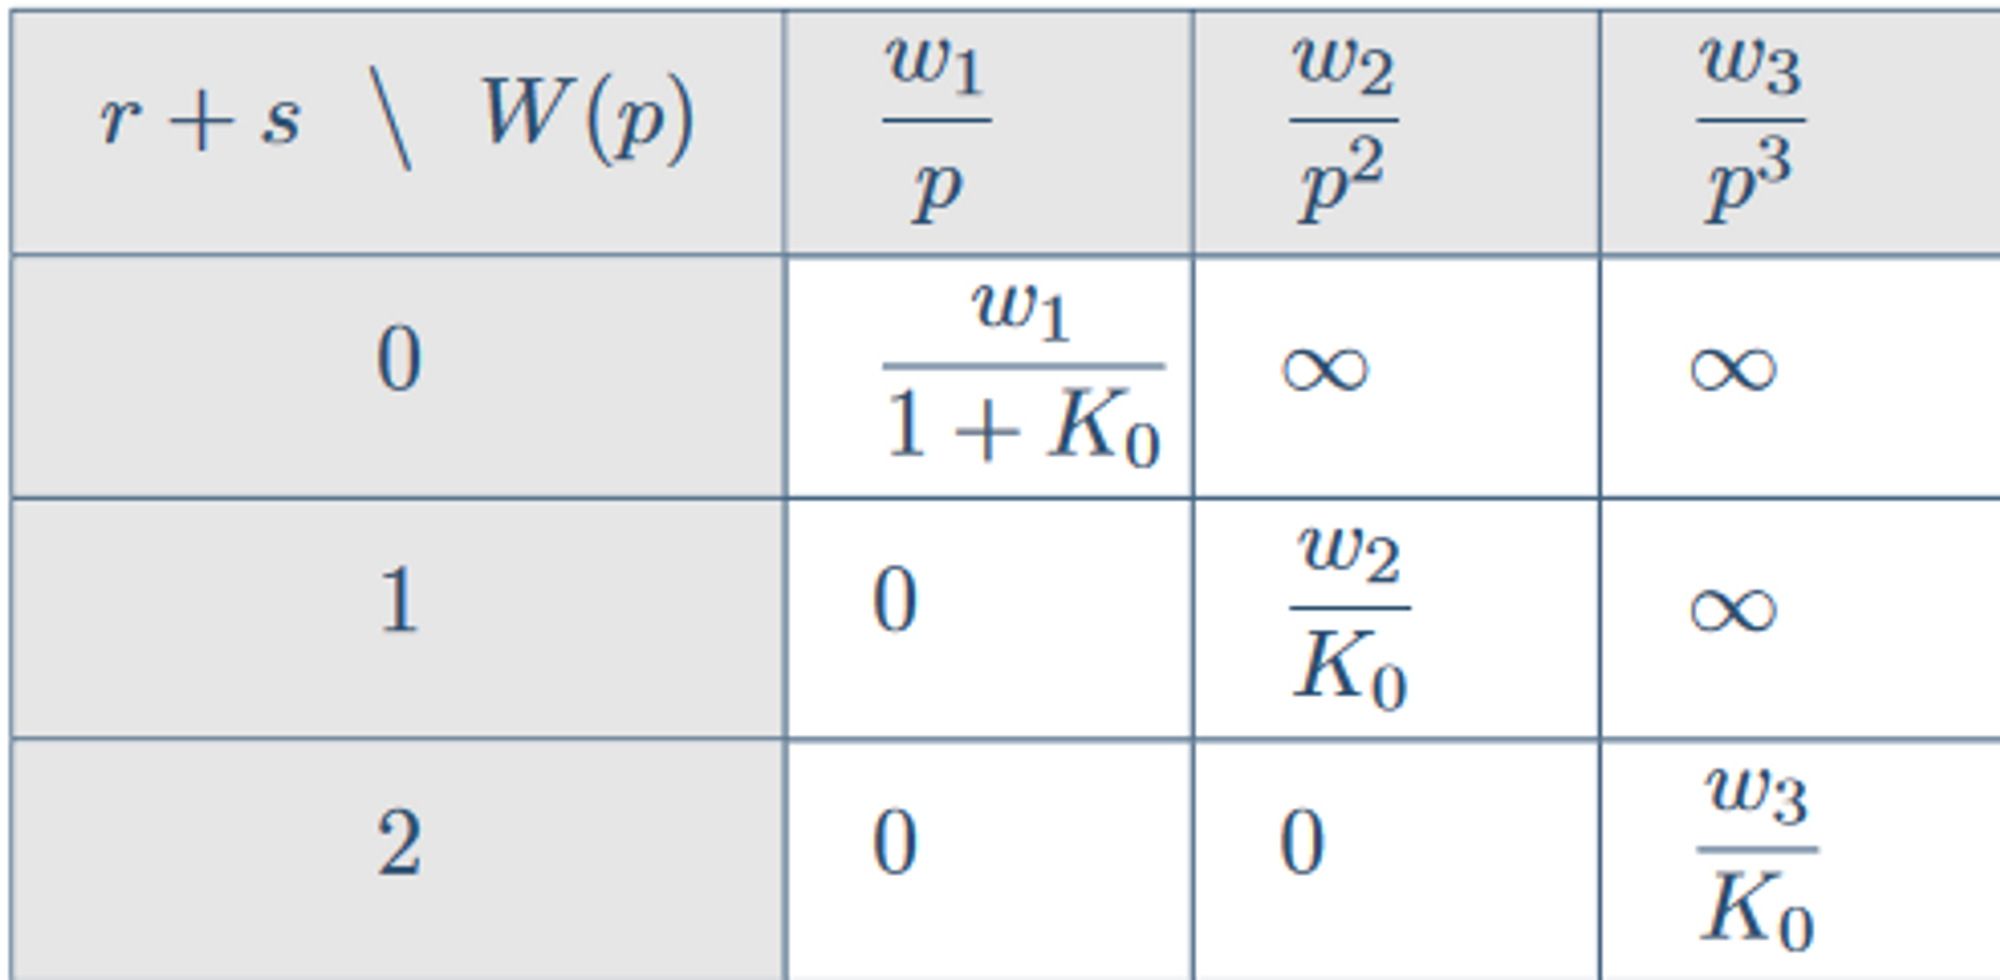
\includegraphics[scale = 0.3]{images/ustalena_odchylka.png}
\end{figure}
\newpage
Ustálená odchylka pro různý typy poruch a počet integrátorů v soustavě a vregulátoru:
\begin{figure}[H]
    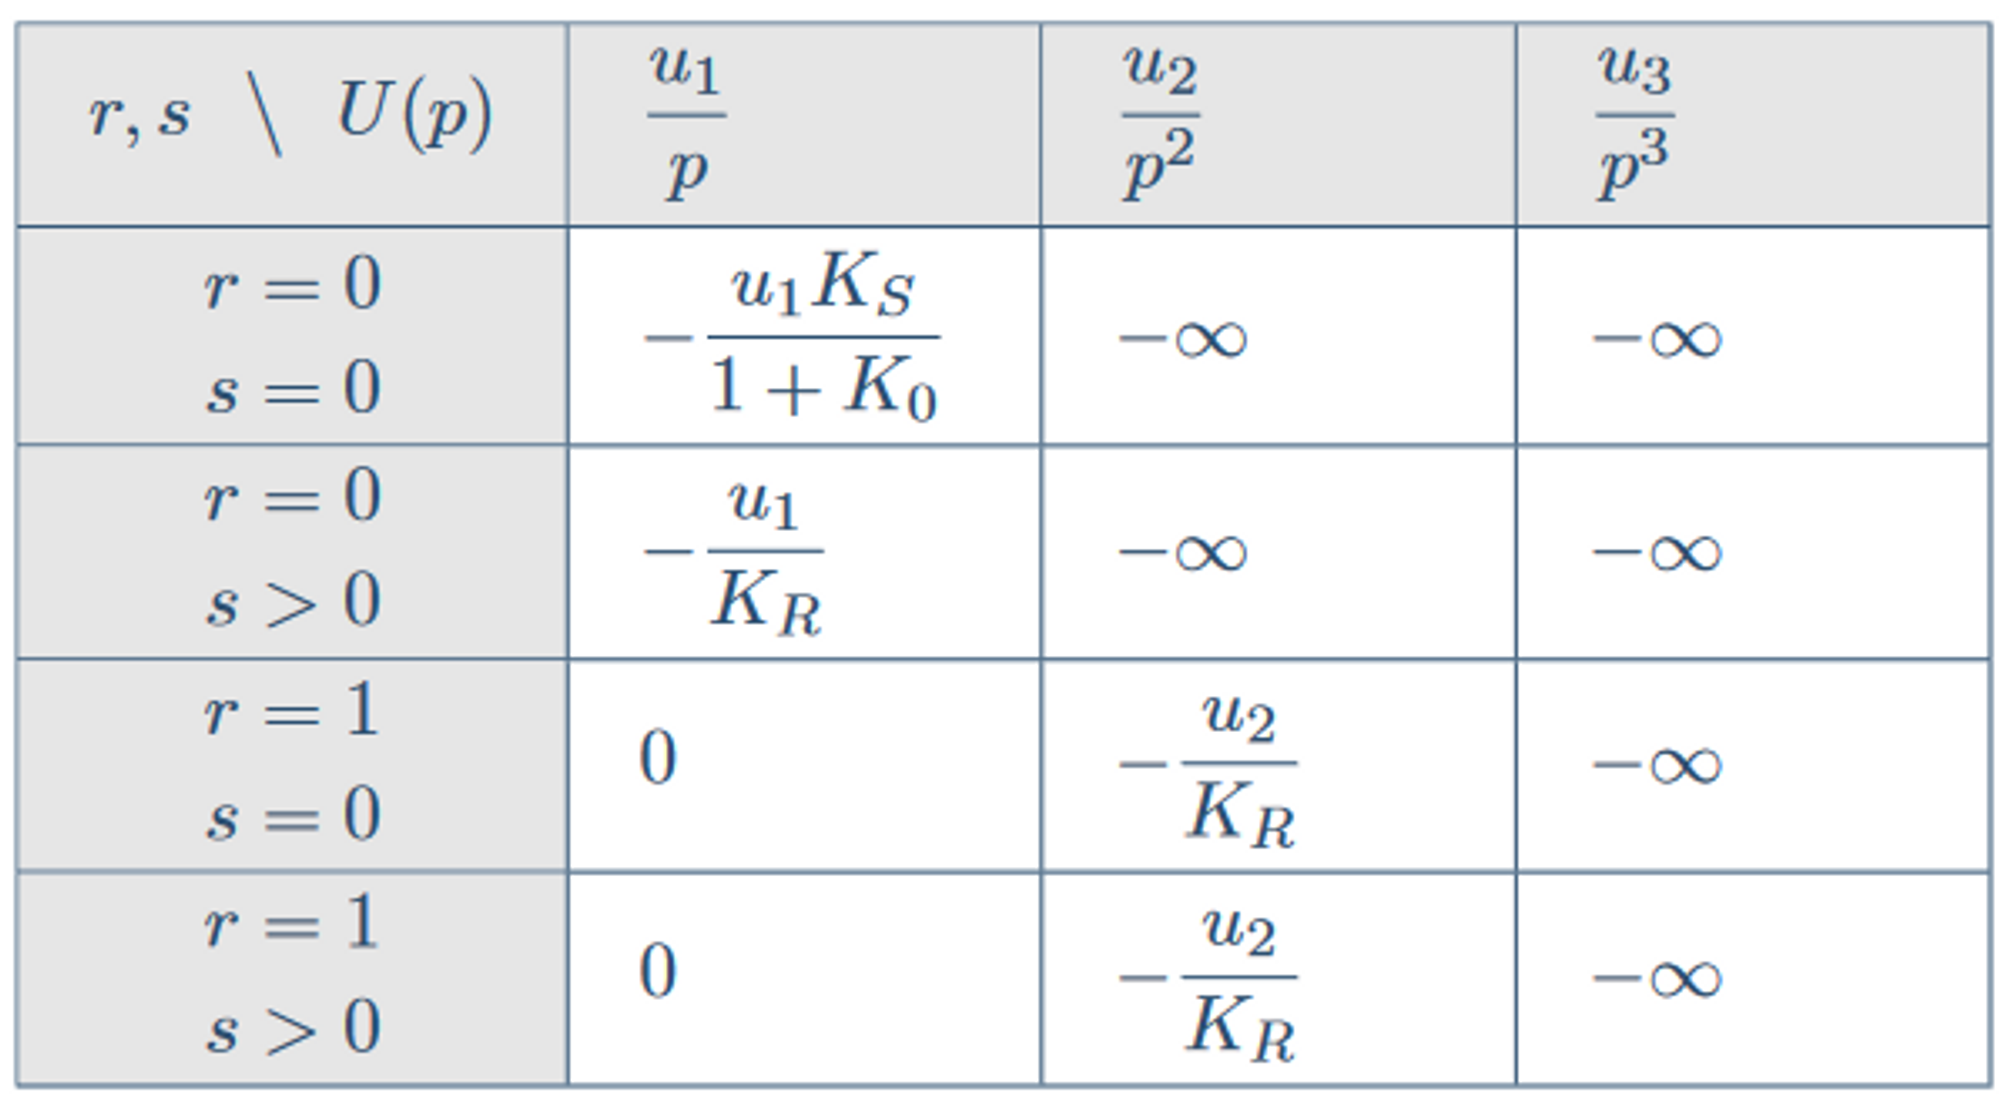
\includegraphics[scale = 0.3]{images/ustalena_odchylka2.png}
\end{figure}
\newpage

\section{Standartní struktury regulačních obvodů. Stabilita obvodů se zpětnou vazbou. Frekvenční charakteristiky v komplexní rovině, Nyquistovo kritérium stability, jeho zjednodušená verze a řešení v logaritmických souřadnicích, použití algebraických kritérií.}
PID:
\begin{figure}[H]
    \includegraphics*[scale = 0.6]{images/PIDschema.png}
\end{figure}


PSD:
\begin{figure}[H]
    \includegraphics*[scale = 0.6]{images/PSDschema.png}
\end{figure}
\newpage

Rozdělení podle stupňů volnosti(kolik regulátorů, tolik stupňů):
\begin{itemize}
    \item jeden stupeň volnosti - odchylkový regulátor
    \begin{figure}[H]
        \includegraphics*[scale = 0.45]{images/jedenStupenVolnostii.png}
    \end{figure}
    \item dva stupňě volnosti(lze plnit požadavky na změnu řízení i poruchy)
    \begin{figure}[H]
        \includegraphics*[scale = 0.4]{images/dvaStupenVolnostii.png}
    \end{figure}
\end{itemize}

\subsection*{Stabilita obvodů se zpětnou vazbou}
Lineární systém je stabilní, pokud výstup po skončení budícího signálu a doznění přechodného děje vrátí na původní hodnotu.\\
Další podmínkou je, když odezva na omezený budící signál je taky omezená, nebo přítomnost všech pólů přenosové funkce v levé polorovině komplexní roviny p(u diskrétních uvnitř jednotkové kružnice).\\

Je několik způsobů, jak určit stabilitu:
\begin{itemize}
    \item Stabilita z charakteristické rovnice
    \item Nyquistovo kritérium stability
    \item Zjednodušené Nyquistovo kritérium
\end{itemize}


\subsubsection*{Stabilita z charakteristické rovnice}
Aby byl zpětnovazební systém stabilní, musí kořeny charakteristické rovnice být v lévé polorovině komplexní roviny p.\\
V charakteristické rovnici se často nachází neznámé proměnné, jsou algebraická kritéria výhodnější(Hurwitz a Routh-Schur).\\

\subsubsection*{Nyquistovo kritérium stability}
Slouží k určení stability uzavřené smyčky.\\
Stabilita se rozhoduje na základě průběhu frekvenční charakteristiky otevřené smyčky a poloze jejich pólů.\\
Využívá se Cauchyho teorému o fázi - mapování uzavřené křivky z roviny p do roviny F.\\
\begin{equation}
    F(p) = \frac{B(p)}{A(p)} = k\frac{(p-\beta_1)(p-\beta_2)\dots (p-\beta_m)}{(p-\alpha_1)(p-\alpha_2)\dots (p-\alpha_m)}
\end{equation}
\begin{figure}[H]
    \includegraphics*[scale = 0.3]{images/NyQuistMapovani.png}
\end{figure}
\textbf{Jestliže uzavřená záporně orientovaná křivka v rovině p obkličuje b nul a a pólů přenosu F(p) a neprochází žádným jejím pólem ani nulou, potom uzavřená křivka vzniklá mapováním obíhá počátek roviny b - a krát v záporném směru}.\\
Pro odvození Cauchyho teorému je důležitá změna fáze uzavřené orientované křivky v rovině F. Fáze přenosu je dána součtem jednotlivých příspěvků kořenových činitelů čitatele $(p - \beta_i)$, od  kterých se odečte součet jednotlivých příspěvků kořenových činitelů jmenovatele $(p - \alpha_i)$.\\
\newpage

Vliv kořenů na změnu fáze uzavřené křivky:
\begin{figure}[H]
    \includegraphics*[scale = 0.3]{images/NyQuistVlivKorenu.png}
\end{figure}
Příspěvek pólů a nul uvnitř křivky je $2\pi$ s tím, že příspěvek pólů se bere se záporným znaménkem.\\
V tomto případě je příspěvek nulový, jelikož pól a nula se odečtou.\\
Využití Cauchyho teorému u Nyquistova kritéria stability:\\
\begin{itemize}
    \item Vytvoření záporně orientované křivky, která obkličuje celou pravou polorovinu roviny p 
    \item Uzavřený systém bude stabilní, pokud bude frekvenční charakteristika pro $\omega = (-\infty, \infty)$ obíhat počátek roviny F v kladném směru tolikrát, kolik nestabilních pólů má přenos F(p)
    \item Jednodušší je sledovat počet oběhů funkce $F_0$ kolem bodu (-1,0)
\end{itemize}
\newpage

Pro případ, kdy máme póly v počátku je nutné je zahrnout buď do pravé, nebo levé poloroviny(zpravidla se zahrnuje do levé, ale funguje na obě strany) - křivka bude pól obcházet s minimálním poloměrem.\\
To že jsme je zahrnuli např. do levé poloroviny neznamená, že jsou stabilní, pouze s nimi v rámci NNyquiistova kritéria jako se stabilními počítáme.\\
\begin{figure}[H]
    \includegraphics*[scale = 0.15]{images/NyQuistPocatek.png}
\end{figure}

\subsubsection*{Zjednodušené Nyquistovo kritérium}
Pokud přenos otevřené smyčky neobsahuje póly v pravé polorovině komplexní roviny p, lze použít zjednodušené Nyquistovo kritérium stability.\\
\begin{figure}[H]
    \includegraphics*[scale = 0.4]{images/NyQuistZjednoduseny.png}
\end{figure}

Uzavřený systém je stabilní, jestli při frekvenci řezu je fáze kladnější, než $-\pi$.\\

\subsubsection*{Algebraické kritéria}
Nevýhodou algebraických kritérií je, že i pro jednoduché příklady vznikají dosti složité řešení.\\
Výhodou je, že dostaneme rozsahy parametrl, pro které je Uzavřený obvod stabilní.\\
Hurwitzuv determinant:
\begin{itemize}
    \item Z charakteristické rovnice se vytvoří čtvercová matice, ze které se určí determinant, který pro stabilitu musí být větší, než 0.
    \begin{figure}[H]
        \includegraphics*[scale = 1.2]{images/Hurwitz.png}
    \end{figure}
    \item Všechny podmínky vycházející z příkladu musí platit společně.
\end{itemize}


Routh-Schurovo kritérium:

\begin{itemize}
    \item všechny koeficienty v redukovaných řádcích musí mět stejné znaménko, aby byl systém stabilní
\end{itemize}
Vzorový příklad k charakteristickému polynomu: $0.1p^5+2.01p^4+10.2p^3+(K_0+1.0)p^2+2.0K_0p+K_0$
\begin{figure}[H]
    \includegraphics*[scale = 1.2]{images/RouthSchur.png}
\end{figure}
\begin{figure}[H]
    \includegraphics*[scale = 1]{images/RouthSchur2.png}
\end{figure}




\section{Analýza dymanických vlastností zpětnovazebních obvodů. Metoda geometrického místa kořenů. Zásoba stability v amplitudě, fázi, modulu. Integrální kritéria kvality regulace, praktická kritéria}
Dynamickými vlastnostmi popisujeme chování systému v přechodných dějích. Tím je myšleno rchlost odeznění, maximální překmit a kmitavost přechodného děje. Neexistuje univerzálně optimálně navrhnutý regulátor, dost záleží na situaci. 
Dynamické vlastnosti se zjišťují z těchto hledisek:
\begin{itemize}
    \item z rozložení nul a pólů v komplexní rovině 
    \item z odezev v časové oblasti
    \item z průběhu frekvenčních charakteristik
\end{itemize}


\subsection*{Metoda kořenového hodografu}
Jedná se o zobrazení průběhu pólů vharakteristické rovnice v závislosti na proměnlivém parametru v komplexní rovině.\\
Postup grafického řešení:
\begin{itemize}
    \item v přenosu otevřené smyčky za p dosdíme p0 jako konkrétní bod 
    \item dále vektor $(p_0 - \alpha_1)$ se dá zapsat v goniometrickém tvaru jako $|p_0 - \alpha_1|\angle (p_0 - \alpha_1)$
    \item fázi získáme tak, že sečtem fáze v čitateli a odečtem fáze ze jmenovatele 
    \item modul je dělení čitatele jmenovatelem
    \item vzorový příklad:
    \begin{figure}[H]
        \includegraphics*[scale = 0.3]{images/hodograf.png}
    \end{figure}
\end{itemize}
\newpage 

\subsubsection*{Soubor pravidel pro konstrukci kořenového hodografu}
\begin{itemize}
    \item Symetrie - kořenový hodograf je symetrucký kolem reálné osy
    \item Počet větví - kořenový hodograf obsahuje n větví 
    \item Segmenty na reálné ose - pokud napravo od části reálné osy leží lichý počet nul a pólů, tak tato část osy je větev kořenového hodografu 
    \item Počátky a konce větví - každá větev začíná při zesílení K = 0 v pólů a končí v k = $\infty$ v nule. Pokud je v přenosu víc pólů, jak nul, tak n - m větví odchází do nekonečna podle přímkových asymptot
    \item Poloha asymptot - asymptoty se protínají na reálné ose v bodě $\sigma = \frac{\sum^n_{i=1} \alpha_i \sum^m_{i=1}\beta_i}{n-m}$ a svírá s kladnou reálnou poloosou úhel $\varphi = \frac{180 \degree + i360\degree}{n - m}$ \dots i = 0, 1 ..., n-m-1
    \item Průsečík s imaginární osou - hodnota K, pro kterou prochází větve kořenového hodografu imaginární osou se dá určit pomocí algebraických kritérií stability
    \item Úhel v komplexní nule nebo pólu - úhel tečny, se kterým vychází větev kořenového hodografu z komplexního pólu $\alpha_k$ se vypočítá jako $\gamma_k = 180 \degree + i360 \degree -\sum^n_{i=1, i\neq k}\angle(\alpha_k - \alpha_i) + \sum^m_{i=1}\angle(\alpha_k - \beta_i)$. Úhel tečny, se kterým vchází větev kořenového hodografu do komplexní nuly $\beta_k$, se vypočítá jako $\delta_k = 180 \degree + i360 \degree -\sum^n_{i=1}\angle(\beta_k - \alpha_i) + \sum^m_{i=1, i\neq k}\angle(\beta_k - \beta_i)$
    \item Průsečík s reálnou osou - průsečík větve kořenového hodografu s reálnou osou se většinou analyticky vyřešit nedá, řeší se iterativně
\end{itemize}
\subsection*{Zásoba stability v amplitudě, ve fázi a v modulu}
\subsubsection*{Zásoba stability v amplitudě}
Hodnota zesílení, se kterou když vynásobíme stávající zesílení otevřené smyčky, tak přivedeme uzavřenou smyčku na mez stability.\\
Udává se ve formě násobícího faktoru nebo v decibelech.\\
Značí se Mg.\\

\subsubsection*{Zásoba stability ve fázi}
Záporně vzatá změna fáze otevřeného obvodu, která přivede uzavřený obvod na mez stability.\\
Značí se Mp.\\

\subsubsection*{Zásoba stability v modulu}
Nejkratší vzdálenost frekvenční charakteristiky otevřené smyčky do bodu -1 v komplexní rovině.\\
Silnější kritérium než Mg a Mp.\\

\begin{figure}[H]
    \centering
    \includegraphics*[scale = 1.2]{images/zasobaStabiliity.png}
\end{figure}
\begin{figure}[H]
    \includegraphics*[scale = 1.1]{images/zasobaStabiliityTabulka.png}
\end{figure}


\subsection*{Integrální kritéria kvality regulace, praktická kritéria}
Výčet kritérií:
\begin{itemize}
    \item Lineární
    \item Usměrněné lineární 
    \item Kvadratické
    \item ITAE
\end{itemize}
\newpage 

\subsubsection*{Lineární}
Odečtení ustálené odchylky zajišťuje konvergenci integrálu k nějaké konečné hodnotě.\\
\begin{equation}
    J_L = \int^\infty_0[e(t) - e(\infty)]dt
\end{equation}
Musí se dodržet, že celá odchylka se pohybuje v kladné hodnotě, jinak nemá smysl, proto se moc nepoužívá.\\
\begin{figure}[H]
    \includegraphics*[scale = 0.3]{images/linearniKriterium.png}
\end{figure}

\subsubsection*{Usměrněné lineární kritérium}
Dá se člen integrálu do absolutní hodnoty.\\
Problém nelinearita u středu.
\begin{equation}
    J_{UL} = \int^\infty_0|e(t) - e(\infty)|dt
\end{equation}
\begin{figure}[H]
    \includegraphics*[scale = 0.3]{images/usmerneneLinearniKriterium.png}
\end{figure}

\subsubsection*{Kvadratické kritérium}
Člen integrálu se dá na druhou.\\
Problém optimální průběhy jsou hodně kmitavé.\\
Přisuzuje se větší váha větším odchylkám.\\
\begin{equation}
    J_K = \int^\infty_0[e(t) - e(\infty)]^2dt
\end{equation}
\begin{figure}[H]
    \includegraphics*[scale = 0.3]{images/kvadratickeKriterium.png}
\end{figure}
\newpage
Existuje analytické řešení - Nekolneho doplněk:
\begin{figure}[H]
    \includegraphics*[scale = 1]{images/nekolnehoDoplnek.png}
\end{figure}
\newpage

\subsubsection*{ITAE kritérium}
Nejpoužívanější\\
Nedá se řešit analyticky.\\
\begin{figure}[H]
    \includegraphics*[scale = 0.3]{images/ITAE.png}
\end{figure}
Zhodnocení vlastností:
\begin{itemize}
    \item méně kmitavý průběh ve srovnání s kvadratickým
    \item váhové kritérium - váha odchylky narůstá s časem
    \item analytický výpočet prakticky nemožný, řešení simulace
\end{itemize}


